%%%%%%%%%%%%%%%%%%%%%%%%%%%%
% CHAPTER                  %
%%%%%%%%%%%%%%%%%%%%%%%%%%%%

\section{L’enjeu de la détection des menaces}
\label{chap2:section1}
{\fontsize{14pt}{16pt}\selectfont
    %%%%%%%%%%%%%%%%%%%%%%%%%%%%
% SECTION                  %
%%%%%%%%%%%%%%%%%%%%%%%%%%%%
\vspace{0.75em}

Les cyberattaques représentent l'une des menaces les plus sérieuses pour les institutions publiques et les entreprises privées. Les attaquants, qu'il s'agisse de pirates informatiques ayant des objectifs malveillants ou d'agents étatiques, utilisent des méthodes de plus en plus sophistiquées pour s'infiltrer dans les systèmes, voler des données sensibles, perturber les opérations et causer des dommages financiers et/ou des atteintes à la réputation. \hyperref[biblio]{[8]}\\

Ces acteurs malveillants poursuivent l’amélioration constante de leurs capacités à des fins de gain financier, d’espionnage ou encore de déstabilisation. Cette amélioration s’illustre en particulier dans le ciblage des  attaquants qui cherchent à obtenir des accès discrets et pérennes aux réseaux de leurs victimes. Les acteurs malveillants tentent de compromettre des équipements périphériques qui  leur offrent un accès plus furtif et persistant. Ce ciblage périphérique se transpose également dans le type d’entités attaquées et confirme l’intérêt des attaquants pour les prestataires, les fournisseurs, les sous-traitants, les organismes de tutelle et l’écosystème plus large de leurs cibles finales.\\

Cette amélioration continue des stratégies et des compétences des attaquants met en évidence les limites de la sécurité des réseaux. La mise en place d'architectures sécurisées (pare-feu, antivirus, réseaux locaux virtuels, etc.) ne garantit pas qu'une intrusion informatique soit impossible. Face à des attaquants suffisamment motivés, une erreur humaine ou une vulnérabilité encore inconnue (dite Zero-Day) finira par permettre une intrusion sur le réseau défendu ou sur celui d'un partenaire dont le réseau dépend, quelle que soit la qualité de la sécurité mise en place.\\

Cette faiblesse intrinsèque de la sécurité informatique rend obligatoire la mise en place, au sein des infrastructures numériques sécurisées, d'outils capables de gérer la possibilité que l'infrastructure défendue soit déjà compromise. C'est le rôle que jouent les systèmes de détection d'intrusion en permettant la détection des tentatives d'intrusion au sein d'un réseau supervisé. \hyperref[biblio]{[5]}
}

\newpage

\section{Les systèmes de détection d’intrusion}
\label{chap2:section2}
{\fontsize{14pt}{16pt}\selectfont
    %%%%%%%%%%%%%%%%%%%%%%%%%%%%
% SECTION                  %
%%%%%%%%%%%%%%%%%%%%%%%%%%%%
\vspace{1em}

La détection des intrusions consiste à surveiller les événements qui se produisent dans un système ou un réseau informatique et à les analyser pour y déceler des signes d'intrusion, définis comme des tentatives pour compromettre la confidentialité, l'intégrité, la disponibilité ou pour contourner les mécanismes de sécurité d'un ordinateur ou d'un réseau.\\

Les intrusions sont causées par des attaquants qui accèdent aux systèmes depuis l'internet, par des utilisateurs autorisés des systèmes qui tentent d'obtenir des privilèges supplémentaires pour lesquels ils ne sont pas autorisés, et par des utilisateurs autorisés qui abusent des privilèges qui leur sont accordés. Les systèmes de détection d'intrusion (IDS) sont des produits logiciels ou matériels qui automatisent ce processus de surveillance et d'analyse.\\ 

Un IDS peut être configuré pour surveiller différents types de trafic, tels que les paquets de données, les connexions réseau, les logs de systèmes, etc. Lorsqu'il détecte une activité suspecte, l'IDS génère une alerte qui est envoyée, permettant de prendre des mesures pour bloquer l'attaque ou corriger la vulnérabilité. \hyperref[biblio]{[3]}\\

\vspace{1em}

\subsection{Types d'IDS }

\vspace{1em}

La façon la plus courante de classer les IDS est de les regrouper par source d'information. Certains IDS analysent les paquets du réseau, capturés à partir des flux passants au sein du réseau pour trouver les attaquants. D'autres IDS analysent les sources d'information générées par les systèmes d'exploitation ou les logiciels d'application présents sur les postes utilisateurs pour y trouver des signes d'intrusion. \hyperref[biblio]{[6 - 7]}

\vspace{1em}

\subsubsection{Les systèmes de détection d'intrusion réseau}

\vspace{0.5em}

La majorité des systèmes commerciaux de détection d'intrusion sont basés sur les réseaux. Ces systèmes de détection d'intrusion réseau (ou NIDS : Network Intrusion Detection System) détectent les attaques en capturant et en analysant les paquets du réseau. À l'écoute d'un segment de réseau ou d'un commutateur, un système de détection d'intrusion en réseau peut surveiller le trafic réseau affectant plusieurs hôtes connectés au segment de réseau.\\

\newpage

\begin{figure}[h]%
    \center%
    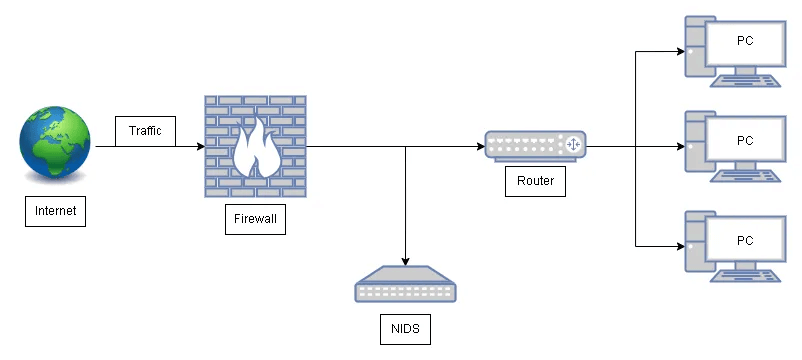
\includegraphics[width=0.9\textwidth]{assets/NIDS.png}
    \caption[Exemple de systèmes de détection d'intrusion réseau (NIDS) (source: \href{https://miro.medium.com/v2/resize:fit:4800/format:webp/1*Jbw1iMzBztCaUokJnqePBg.png}{techno-skills.com})]{Exemple de systèmes de détection d'intrusion réseau (NIDS)}\label{fig:NIDSexemple}
\end{figure}

\vspace{1em}

\textit{Avantages des IDS en réseau :}\\

\begin{itemize}[itemsep=1em]
    \item[•] Quelques IDS bien placés peuvent surveiller un grand réseau ;
    \item[•] Le déploiement d'IDS en réseau a peu d'impact sur un réseau existant. Les IDS basés sur le réseau sont généralement des dispositifs passifs qui écoutent sur un fil de réseaux sans interférer avec le fonctionnement normal d'un réseau ;
    \item[•] Les IDS en réseau peuvent être configurés de manière à être hautement sécurisés contre les attaques et très difficiles à détecter pour les attaquants.\\
\end{itemize}

\vspace{1em}

\textit{Inconvénients des IDS en réseau :}\\

\begin{itemize}[itemsep=1em]
    \item[•] Les IDS basés sur le réseau peuvent avoir des difficultés à traiter tous les paquets dans un réseau important ou très fréquenté et, par conséquent, ne pas reconnaître une attaque lancée pendant les périodes de fort trafic ;
    \item[•] Les IDS basés sur le réseau ne peuvent pas analyser les informations chiffrées. Ce problème s'aggrave car de plus en plus d'organisations (et d'attaquants) utilisent des réseaux privés virtuels ;
    \newpage
    \item[•] La plupart des IDS basés sur le réseau ne peuvent pas déterminer si une attaque a réussi ou non ; ils peuvent seulement discerner qu'une attaque a été initiée. Cela signifie qu'après la détection d'une attaque par un système IDS basé sur le réseau, un examen manuel (ou une corrélation automatique à l'aide d'autres sources de données comme des logs) devra être effectué afin de caractériser si l'attaque a été réussie.
\end{itemize}

\vspace{1em}

\subsubsection{Systèmes de détection d'intrusion au niveau de l'hôte}

\vspace{0.5em}

Les systèmes de détection d'intrusion au niveau de l'hôte (ou HIDS : Host-based Intrusion Detection System), reposant sur l'hôte, fonctionnent sur la base des informations collectées à l'intérieur des appareils des utilisateurs. Les IDS basés sur l'hôte utilisent normalement des sources d'information de deux types : les pistes d'audit du système d'exploitation et les journaux du système. Ils permettent également de prendre un instantané des fichiers système existants et de les comparer à l'instantané précédant pour générer des alertes en cas de modifications.\\

\vspace{1em}

\begin{figure}[h]%
    \center%
    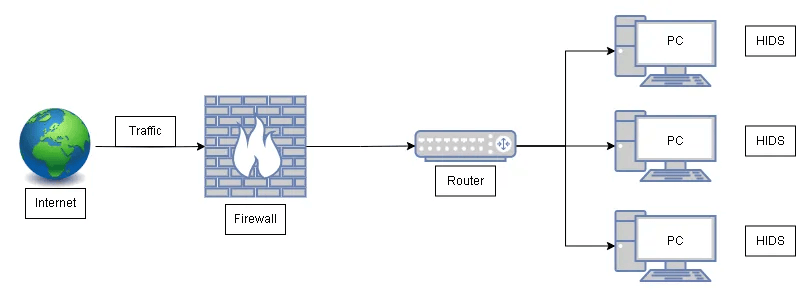
\includegraphics[width=0.9\textwidth]{assets/HIDS.png}
    \caption[Exemple de systèmes de détection d'intrusion au niveau de l'hôte (HIDS) (source: \href{https://miro.medium.com/v2/resize:fit:4800/format:webp/1*Jbw1iMzBztCaUokJnqePBg.png}{techno-skills.com})]{Exemple de systèmes de détection d'intrusion au niveau de l'hôte (HIDS)}\label{fig:HIDSexemple}
\end{figure}

\vspace{1em}

\textit{Avantages des IDS basés sur les hôtes :}\\

\begin{itemize}[itemsep=1em]
    \item[•] Les IDS basés sur l'hôte, grâce à leur capacité à surveiller les événements locaux d'un hôte, peuvent détecter des attaques qui ne peuvent l'être par un IDS basé sur le réseau ;

\newpage

    \item[•] Les IDS basés sur l'hôte peuvent fonctionner dans un environnement où le trafic réseau est chiffré, les sources d'information étant générées avant le chiffrement des données et/ou après le déchiffrement des données sur l'hôte de destination ;
    \item[•] Les IDS basés sur l'hôte ne sont pas affectés par les réseaux commutés.\\
\end{itemize}

\vspace{1em}

\textit{Inconvénients des IDS basés sur les hôtes :}\\
\vspace{0.5em}
\begin{itemize}[itemsep=1em]
    \item[•] Les IDS basés sur l'hôte sont plus difficiles à gérer, car les informations doivent être configurées et gérées pour chaque hôte surveillé ;
    \item[•] Étant donné que les sources d'information des IDS basés sur l'hôte résident sur l'hôte ciblé par les attaques, l'IDS peut être attaqué et désactivé dans le cadre de l'attaque ;
    \item[•] Les IDS basés sur l'hôte ne sont pas bien adaptés à la détection des scans de réseau ou d'autres formes de surveillance ciblant l'ensemble d'un réseau, car l'IDS ne voit que les paquets de réseau reçus par son hôte.
\end{itemize}

\newpage

\subsection{Méthode de détection }

\vspace{1em}

Les technologies IDS utilisent de nombreuses méthodologies pour détecter les incidents. Ces méthodologies peuvent être regroupées en deux grandes catégories : celles basées sur les signatures et celles basées sur les anomalies.  La plupart des technologies IDS utilisent plusieurs méthodologies de détection, séparément ou intégrées, afin de fournir une détection plus large et plus précise. \hyperref[biblio]{[1]}

\subsubsection{Les IDS à base de signatures}
\label{chap2:IDSsignature}

\vspace{0.5em}

Les IDS à base de signatures ont une base de données comportant un ensemble de signatures d’attaques (base de signatures). Le principe de fonctionnement est le test de correspondance. Les données du réseau sont analysées et comparées aux signatures d’attaques connues stockées dans la base de signatures. En cas de correspondance, une alerte est émise. Un avantage de ce système est qu’il a une meilleure précision lorsque les règles de signature sont correctes. Cette base de signatures est en général pré-initialisée avec des données de l’éditeur de l’IDS et mise à jour régulièrement pour prendre en compte les nouvelles attaques.\\

La détection basée sur les signatures est très efficace pour détecter les menaces connues, mais largement inefficace pour détecter les menaces inconnues. Elle a l'avantage d'être facile à mettre en place, mais sa principale limite est que si l'attaquant est conscient des règles de détection en place, il peut modifier légèrement sa technique pour qu'elle ne soit plus détectable.\\

\begin{figure}[h]%
    \center%
    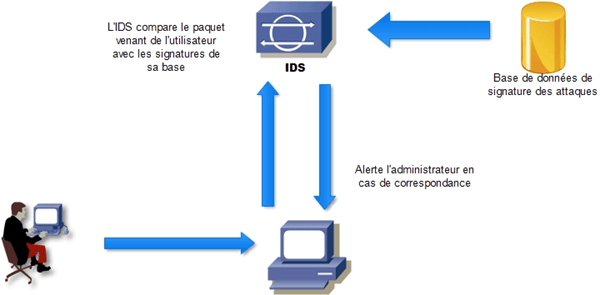
\includegraphics[width=0.9\textwidth]{assets/IDSbaseSignatures.png}
    \caption[Procédure de détection d’attaques d’un IDS à base de signatures (source: \href{https://techno-skills.com/wp-content/uploads/2020/12/image-4.png}{techno-skills.com})]{Procédure de détection d’attaques d’un IDS à base de signature}\label{fig:ids-signature}
\end{figure}

\newpage

\subsubsection{Les IDS à base d’anomalies}

\vspace{0.5em}

Cette catégorie d’IDS utilise un modèle statistique du fonctionnement de référence du réseau qui peut comprendre la bande passante utilisée, les protocoles définis pour le trafic, les ports et les périphériques qui font partie du réseau. Il surveille régulièrement le trafic réseau et le compare au modèle statistique. En cas d’anomalie ou de divergence, l’administrateur est alerté. Un avantage de ce système est qu’il peut détecter des attaques nouvelles dont le comportement s’éloigne suffisamment de la normale.\\

Malheureusement, les détecteurs d'anomalies et les systèmes de détection d'intrusion qui en découlent produisent souvent un grand nombre de fausses alertes, car les modèles normaux de comportement des utilisateurs et des systèmes peuvent varier considérablement sans être prévisibles. Ce type de détection est difficile à utiliser de manière efficace.\\

\begin{figure}[h]%
    \center%
    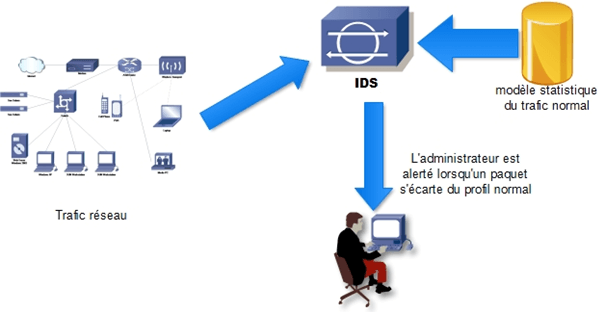
\includegraphics[width=0.9\textwidth]{assets/IDSbaseAnomalies.png}
    \caption[Procédure de détection d’attaques d’un IDS à base d’anomalies (source: \href{https://techno-skills.com/wp-content/uploads/2020/12/image-5.png}{techno-skills.com})]{Procédure de détection d’attaques d’un IDS à base d’anomalies}\label{fig:ids-anomalie}
\end{figure}

\subsubsection{\textit{Note}}
Dans le cadre de mes travaux, j'ai travaillé avec des systèmes de détection d'intrusion réseaux faisant de la détection par signatures. Ce choix technologique se justifie dans le contexte de l'AMSN par le besoin de posséder une capacité de détection pouvant fonctionner sur les réseaux de tous les OIV en même temps sans perturber leurs activités usuelles. L'utilisation de la détection à base d’anomalies et des Systèmes de détection d’intrusion au niveau de l’hôte serait beaucoup plus difficile par la diversité des OIV et demanderait un niveau de connaissance sur les réseaux supervisés que l'Agence n'a pas vocation à connaître.
}

\newpage

\section{Les indicateurs de compromission}
\label{chap2:section3}
{\fontsize{14pt}{16pt}\selectfont
    %%%%%%%%%%%%%%%%%%%%%%%%%%%%
% SECTION                  %
%%%%%%%%%%%%%%%%%%%%%%%%%%%%
\vspace{1em}

Les IDS, notamment ceux faisant de la détection par signatures, ont besoin d'une base de référentiels pour savoir quoi détecter. C'est ce rôle que jouent les indicateurs de compromission (ou IOC : Indicator Of Compromise)\\

Un indicateur de compromission, en sécurité informatique, est une déviance ou un artéfact observé sur un réseau ou dans un système d'exploitation qui indique, avec un niveau de certitude déterminé, une intrusion informatique. Des indicateurs de compromission peuvent être : des signatures virales, des adresses IP particulières, des hachages de fichiers malveillants, des URLs ou des noms de domaine de serveurs de commande et de contrôle de botnets, etc. \hyperref[biblio]{[4]}\\

\begin{figure}[h]%
    \center%
    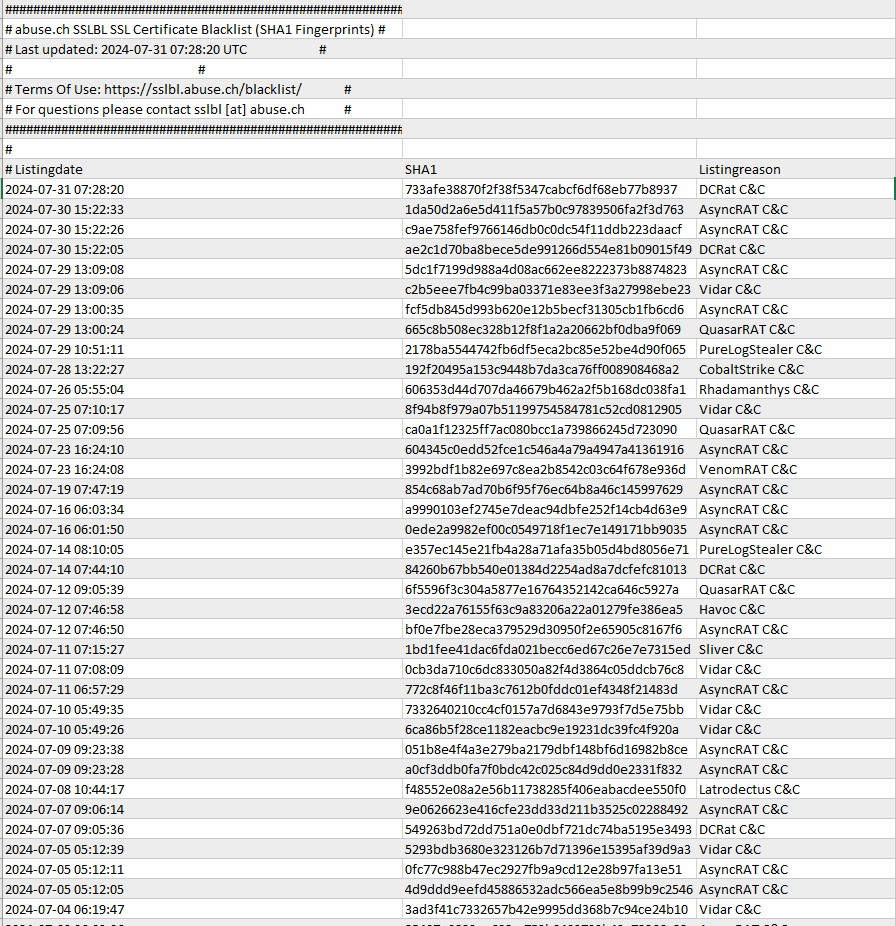
\includegraphics[width=0.74\textwidth]{assets/IOC.png}
    \caption[Exemple de liste d'IOC de hachages de fichiers malveillants fournie par \textit{abuse.ch} (source: \href{https://sslbl.abuse.ch/blacklist/sslblacklist.csv}{sslbl.abuse.ch/blacklist/sslblacklist.csv})]{Exemple de liste d'IOC de hachages de fichiers malveillants fournie par \textit{abuse.ch}}\label{fig:ioc}
\end{figure}

\newpage

Ces IOC sont découverts à la suite d'investigations numériques (également appelées renseignements sur les menaces ou \textit{threat intelligence}) menées sur les traces laissées par des acteurs malveillants en ligne ou à partir d'une analyse post-incident des techniques utilisées par les attaquants qui ont tenté ou réussi à pénétrer dans le système informatique. Ces IOC sont ensuite partagés par différents acteurs:\\

\begin{itemize}[itemsep=1em]
    \item[•] \textbf{Organismes de cybersécurité}\\
    La plupart des CERT étatiques (CERT-FR Français, US-CERT Américains, etc.) ou privés (CERT Orange, CERT Crédit Agricole, etc.) réalisent en partie eux-mêmes de la collecte d'IOC qu'ils partagent en privé entre agences lorsque des accords de collaboration existent, mais aussi publiquement pour une part\footnote{Exemple source publique du CERT-FR: \url{https://www.cert.ssi.gouv.fr/ioc/}}.
    \item[•] \textbf{Entreprises spécialisées de CTI}\\
    Le besoin de renseignement sur les menaces existantes ne cessant de croître, des sociétés spécialisées se sont créées pour répondre à cette demande (CrowdStrike, Sekoia.io, etc.) en plus des autres services de cybersécurité qu'elles peuvent pourvoir. En échange d'un contrat rémunéré, ces sociétés fournissent des listes d'IOC régulièrement mises à jour.
    \item[•] \textbf{Plate-formes d'échange libre de renseignement cyber}\\
    Pour faire face à l'ampleur des menaces, des plateformes de coopération CTI ont commencé à apparaître en ligne, impliquant des organisations étatiques et privées ainsi que des professionnels individuels du secteur. Grâce à ces plateformes (MISP, alienvault, threatfox, etc.), les utilisateurs peuvent s'alerter mutuellement des évènements cyber en cours et partager les IOC qu'ils possèdent.
\end{itemize}
}

% \begin{itemize}
% 	\item The individual \index{Entries}{entries} are indicated with a black dot, a so-called bullet.
% Tout au long de ces périodes, Bruno VALENTIN et Sébastien ABBONDANZA ont suivi mon travail en programmant des rapports bimensuels au cours desquels j'ai régulièrement fait part de mes progrès et reçu des conseils de leur part.\\
% 	\item The text in the entries may be of any length.
% \end{itemize}

% \begin{theorem}\label{theo1}
% Soit $n$ un entier naturel. Si $n$ est premier alors il n'est divisible que par 1 et par lui-même.
% \end{theorem}

% \begin{proof}
% Here is my proof.
% \end{proof}

% \begin{definition}\label{def1}
% Soit $A$ une courbe...
% \end{definition}

% Ici, il s'agit de l'utilisation de TB %\nomenclature[TB]{TB}{Très Bien} qui consiste à parler Très Bien. 
% \gls{abc} et \gls{efg} sont des acronyms et des abbréviations... La méthode \gls{svm} est également couramment utilisée.

% \begin{exemple}\label{exo1}
% On considère le cas particulier... 
% \end{exemple}